\section{Results}
\label{sec:results}
%% Points:
%% - Supervised experiments (table 1) + zero-shot (table 2)
%% - TTDA experiments (table 3)
%% - Some images showing the evolution <-- Save ckpts for some imgs then

\begin{margintable}[]\small
\caption{Number of trainable parameters for each method}
\label{tab:trainable_params}
\begin{tabular}{@{}p{1.75cm}P{2cm}@{}}
\toprule
{Method}       & {Learnable Parameters (M)}\\ \midrule
Fine-Tuning                         & 90.60     \\
Decoder FT                          & 3.92      \\
LoRA~{\footnotesize\parencite{hu2022lora}}              & 4.07      \\
Med-SA~{\footnotesize\parencite{wu2023medical}}         & 11.03     \\
HQ-SAM~{\footnotesize\parencite{ke2024segment}}         & 1.07      \\
SAM-DA                              & 0.66      \\ \bottomrule
\end{tabular}
\end{margintable}

\subsection{Full Supervision}
\Cref{tab:supervised_training} presents a comparison of the IoU scores achieved by SAM Decoder Adapter (SAM-DA) against alternative baselines across four datasets in the fully supervised task. Our approach consistently delivers comparable or superior results to full fine-tuning despite employing only a fraction of the trainable parameters\sidenote{See \Cref{tab:trainable_params}}. Notably, the number of training images influences the model's final performance: the BMC domain in the MRI dataset, with the fewest samples across all datasets, showcases significant performance improvement with our adapter compared to other methods. With fewer parameters, SAM Decoder Adapter is less susceptible to overfit to the training set, thereby retaining valuable knowledge from the pre-trained weights. This effect diminishes as the dataset size increases, where the advantage of the adapter over competitive baselines is less evident. \cref{fig:full_superv} shows qualitative results of our adapter.



Due to the substantial number of images in HQSeg-44K~\sideauthorcite{ke2024segment}, this dataset can be considered quite distinct. With 44k training images, encoder-adaptation methods are expected to outperform decoder-only approaches due to their higher number of parameters. Our method achieves an IoU score of 79.6 on this dataset, falling behind LoRA and Med-SA (with an average IoU of 83.5). However, it surpasses other decoder-only adapters like HQ-SAM, which achieves an IoU of 79.2. These results are the average over the four testing sets in HQSeg-44K, and the detailed figures can be found on \Cref{tab:hqseg_results_samda}.

\begin{table*}
\caption{IoU scores for the full supervision task. Variances are computed over four trained models on the validation set. Bold numbers indicate the best adapter. Asterisks indicate the second best.\label{tab:supervised_training}}
\centering
\begin{tabular}{@{}lP{3.3cm}P{2.5cm}P{2.5cm}P{2.5cm}@{}}
\toprule
  & Retouch - Spectralis & MRI - BMC & WMH - Utrecht & HQSeg-44K  \\ \midrule
Fine-Tuning &  $76.0{\scriptscriptstyle \pm 0.6}$ & $85.9{\scriptscriptstyle \pm 1.5}$ & $43.5{\scriptscriptstyle \pm 0.9}$ & $76.0{\scriptscriptstyle \pm 0.3}$  \\ \midrule
Decoder FT  & $42.8{\scriptscriptstyle \pm 2.0}$ & $71.9{\scriptscriptstyle \pm 2.6}$ & $40.8{\scriptscriptstyle \pm 0.3}$ & $80.9{\scriptscriptstyle \pm 0.3}$  \\
LoRA~\cite{hu2022lora} & $74.1{\scriptscriptstyle \pm 1.1}$ & $83.7{\scriptscriptstyle \pm 1.3}$ & $43.1{\scriptscriptstyle \pm 0.5}$ & $83.1{\scriptscriptstyle \pm 0.3}$*  \\
Med-SA~\cite{wu2023medical}  & $75.0{\scriptscriptstyle \pm 1.2}$* & $84.3{\scriptscriptstyle \pm 1.9}$* & $\mathbf{44.7}{\scriptscriptstyle \pm 0.7}$ & $\mathbf{83.8}{\scriptscriptstyle \pm 0.4}$  \\
HQ-SAM~\cite{ke2024segment}  & $52.4{\scriptscriptstyle \pm 2.1}$ & $76.5{\scriptscriptstyle \pm 1.5}$ & $40.9{\scriptscriptstyle \pm 0.6}$ & $79.2{\scriptscriptstyle \pm 0.2}$  \\ \midrule
SAM-DA  & $\mathbf{75.4}{\scriptscriptstyle \pm 0.6}$ & $\mathbf{86.2}{\scriptscriptstyle \pm 1.5}$ & $44.2{\scriptscriptstyle \pm 0.3}$* & $79.6{\scriptscriptstyle \pm 0.4}$  \\ \bottomrule
\end{tabular}
\end{table*}

\plainwidefig{1}{Figures/full_supervision_MICCAI.pdf}{Qualitative results on eight randomly selected test samples.}{fig:full_superv}

%\input{tables/hqseg_results}

\subsection{Domain Generalization}
One of the primary strengths of SAM lies in its ability to zero-shot transfer thanks to its extensive pre-training corpus. We investigate in \Cref{tab:zero_shot} whether this capability is retained after the adaption by testing the methods from \Cref{tab:supervised_training} on previously unseen domains within each medical dataset. SAM Decoder Adapter demonstrates significant superiority in zero-shot generalization compared to other methods that primarily focus on traditional encoder adaptation, such as Med-SA and LoRA, and shows on-par performance to fine-tuning in the low-data regime. See supplementary material for qualitative results of our adapter compared to two baselines on the generalization domains.

\begin{table}[]
\sidecaption{Domain generalization results on an unseen domain (IoU score). Variances are computed over four trained models on the validation set.\label{tab:zero_shot}}
\centering
\begin{tabular}{@{}lP{2.5cm}P{2.5cm}P{3cm}@{}}
\toprule
 & Retouch - Cirrus & MRI - UCL & WMH - Singapore \\ \midrule
Fine-Tuning & $65.4{\scriptscriptstyle \pm 5.1}$ & $80.9{\scriptscriptstyle \pm 1.1}$ & $40.1{\scriptscriptstyle \pm 0.9}$ \\ \midrule
Decoder FT & $27.0{\scriptscriptstyle \pm 0.7}$ & $70.4{\scriptscriptstyle \pm 0.8}$ & $35.8{\scriptscriptstyle \pm 0.95}$ \\
LoRA~\cite{hu2022lora} & $56.0{\scriptscriptstyle \pm 5.6}$ & $75.9{\scriptscriptstyle \pm 1.5}$ & $37.3{\scriptscriptstyle \pm 1.0}$ \\
Med-SA~\cite{wu2023medical} & $61.7{\scriptscriptstyle \pm 3.5}$ & $75.8{\scriptscriptstyle \pm 7.0}$ & $38.8{\scriptscriptstyle \pm 1.2}$ \\
HQ-SAM~\cite{ke2024segment} & $30.8{\scriptscriptstyle \pm 0.4}$ & $75.8{\scriptscriptstyle \pm 3.7}$ & $35.9{\scriptscriptstyle \pm 0.7}$ \\ \midrule
SAM-DA & $\mathbf{70.2}{\scriptscriptstyle \pm 3.1}$ & $\mathbf{80.6}{\scriptscriptstyle \pm 1.0}$ & $\mathbf{39.6}{\scriptscriptstyle \pm 0.7}$ \\ \bottomrule
\end{tabular}
\end{table}

%We attribute the significant generalization capability of our method to its focus on adapting the decoder only, and prove it by applying it to the encoder. Unlike other approaches that prioritize encoder adaptation, necessitating decoder training, our method leverages pre-trained weights, yielding an already proficient decoder.


% - Locating the adapter in the encoder: show all the tables but only compare the encoder adapter to ours.

%We extensively analyze the proposed adapter through detailed ablation studies, using ViT-B as the backbone and measuring the impact of the adapter's position.
\subsection{Ablation study}\label{sec:ablation_samda}
The Vision Transformer-type architecture used in the backbone of SAM facilitates the seamless integration of the proposed adapter into the encoder with minimal adjustments compared to the configuration depicted in \cref{fig:method_samda}. We adopt the approach outlined in \yeartextcite{llama_adapter} to position the adapter within the encoder, focusing on adapting only the last layers. Additionally, we utilize all image embeddings as queries for the attention module and fine-tune the decoder, following the setting from LoRA and Med-SA. ViT-B comprises 12 blocks, and we modify the last ten blocks in our adaptation approach. This adaptation strategy allocates $17.7$M trainable parameters to the encoder adaptation, in addition to $3.9$M parameters in the decoder. \Cref{tab:encoder_ablation_trained,tab:encoder_ablation_generalization} illustrate the impact of adapting the encoder layers compared to the proposed method. The results confirm that locating the adapter in the decoder improves generalization on unseen domains\sidenote{As seen in \Cref{tab:encoder_ablation_generalization}.}, especially in the case of Retouch and WMH datasets, where we see a gain of $8.5\%$ and $13.8\%$ in IoU score, respectively.

\begin{table*}[]
\caption{Ablation study evaluating two adapter locations. IoU scores for full supervision. Variances are obtained over four trained models on the validation set.}
\label{tab:encoder_ablation_trained}
\centering
\begin{tabular}{@{}lP{3.3cm}P{2.5cm}P{2.5cm}P{2.5cm}@{}}
\toprule
 & Retouch - Spectralis & MRI - BMC & WMH - Utrecht & HQSeg-44K  \\ \midrule
Decoder Adapter & $75.4{\scriptscriptstyle \pm 0.6}$ & $\mathbf{86.2}{\scriptscriptstyle \pm 1.5}$ & $\mathbf{44.2}{\scriptscriptstyle \pm 0.3}$ & $79.6{\scriptscriptstyle \pm 0.4}$ \\
Encoder Adapter & $\mathbf{75.8}{\scriptscriptstyle \pm 1.0}$ & $84.6{\scriptscriptstyle \pm 2.2}$ & $40.7{\scriptscriptstyle \pm 0.3}$ & $\mathbf{80.8}{\scriptscriptstyle \pm 0.3}$ \\ \bottomrule 
\end{tabular}
\end{table*}

\begin{table}[]
\sidecaption{Ablation study evaluating two adapter locations. IoU scores for domain generalization. Variances are obtained over four trained models on the validation set.\label{tab:encoder_ablation_generalization}}
\centering
\begin{tabular}{@{}lP{3cm}P{2.5cm}P{3cm}@{}}
\toprule
 & Retouch - Cirrus & MRI - UCL & WMH - Singapore  \\ \midrule
Decoder & $\mathbf{70.2}{\scriptscriptstyle \pm 3.1}$ & $\mathbf{80.6}{\scriptscriptstyle \pm 1.0}$ & $\mathbf{39.6}{\scriptscriptstyle \pm 0.7}$ \\
Encoder & $64.7{\scriptscriptstyle \pm 6.8}$ & $80.4{\scriptscriptstyle \pm 1.4}$ & $34.8{\scriptscriptstyle \pm 0.6}$ \\ \bottomrule

\end{tabular}
\end{table}

\subsection{Test-Time Domain Adaptation}
Due to the low number of trainable parameters, test-time domain adaptation is the ideal setting to test how much an adapter can affect the performance of a single test sample. We show in \Cref{tab:ttda} that our adapter performs better than other baselines in most cases. For MRI, the increase in trainable parameters already in LoRA hurts the initial model and decreases its IoU score after only five iterations. Our method, however, shows strong results in all three cases, as shown in \Cref{fig:ttda_samda} in the appendix.

%In Fig. \ref{fig:ttda}, we compare two runs for Retouch and MRI between our adapter and LoRA (the second best).

\begin{table}[]
\sidecaption{Test-time domain adaptation results (IoU score). Due to the challenge of zero-initializing HQ-SAM, we omit it from these experiments.\label{tab:ttda}}
\centering
\begin{tabular}{@{}lP{2.5cm}P{2.5cm}P{3cm}@{}}
\toprule
 & Retouch - Cirrus & MRI - UCL & WMH - Singapore \\ \midrule
Fine-Tuning & 61.2 & 80.2 & 39.6 \\
Decoder FT & 66.9 & 80.8 & 40.4 \\
LoRA~\cite{hu2022lora} & 67.0 & 80.7 & 40.3 \\
Med-SA~\cite{wu2023medical} & 63.3 & 80.7 & 40.4 \\ \midrule
%HQ-SAM~\cite{ke2024segment} & - & - & - \\ \midrule
SAM-DA & \textbf{67.5} & \textbf{81.1} & \textbf{40.4} \\ \bottomrule
\end{tabular}
\end{table}

%\begin{figure}
%\centering
%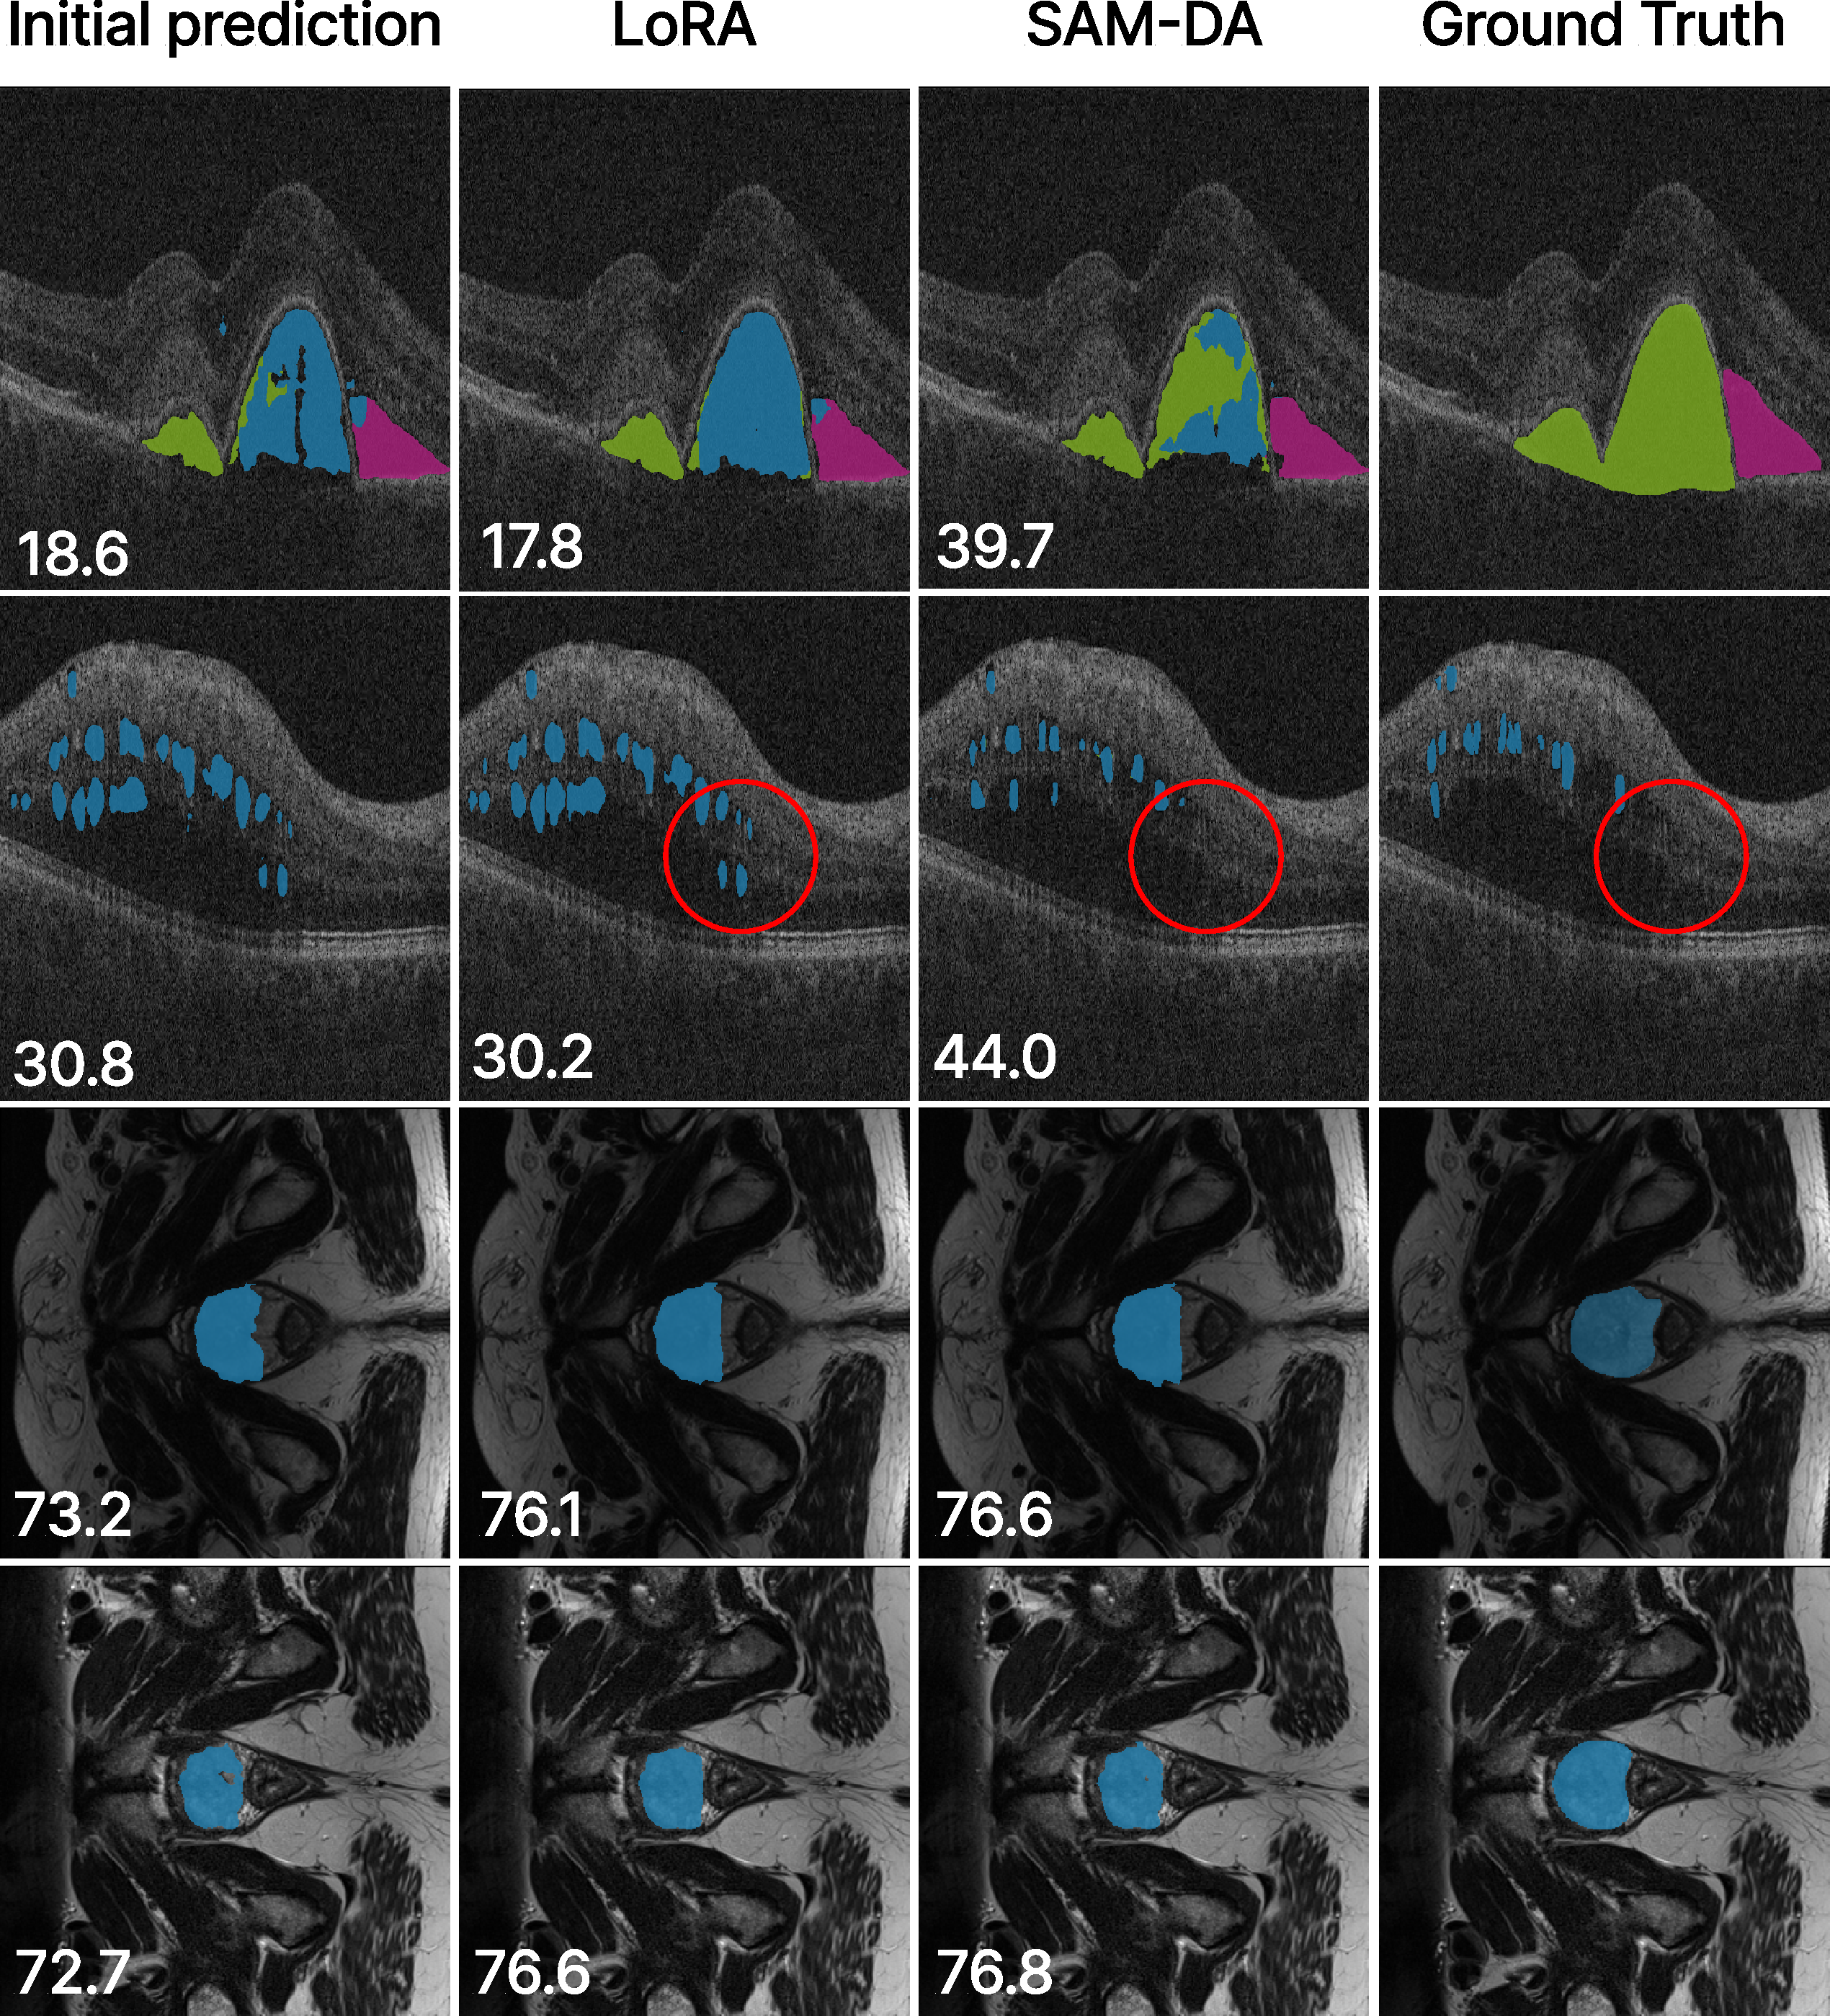
\includegraphics[width=\textwidth]{ttda.pdf}
%\caption{Qualitative and quantitative results on Retouch and MRI datasets for the proposed model and LoRA. For reference, each image has its IoU score after five TTDA iterations.
%}
%\label{fig:ttda}
%\end{figure}

